\documentclass[twoside]{mfitjournal}
\usepackage{amsbib}
\usepackage[T2A]{fontenc}
\usepackage[utf8]{inputenc}
\usepackage[russian]{babel}
\usepackage{amsmath,amssymb}
\usepackage{graphicx}
\usepackage{geometry}
\usepackage{array}
\usepackage{booktabs}
\usepackage{caption}
\usepackage{float}
\usepackage{needspace}
\clubpenalty=10000
\widowpenalty=10000
\newcommand{\MFITnumber}{}
\newcommand{\MFITom}{}
\newcommand{\MFITyear}{2026}
\newcommand{\ISSN}{}
\newcommand{\OISSN}{}
\newcommand{\DOI}{}
\renewcommand{\firstpage}{}
\renewcommand{\lastpage}{}
\SECC{}
\ESECC{}
\geometry{margin=2cm}
\newcommand{\degree}{$^\circ$}
\setlength{\headheight}{15pt}
\captionsetup{font=small, labelfont=bf}

\begin{document}

\rustitle{Лабораторная работа 4.5.2. Интерференция лазерного излучения}
\shorttitle{Лабораторная работа 4.5.2}
\author{Евгений Иванов}
\shortauthor{Иванов Е.\,И.}
\institute{МФТИ, группа 5-407}
\email{}{}
\rcopyr{Евгений Иванов}

\makeatletter
\renewcommand{\tit}{}
\renewcommand{\@oddhead}{}
\renewcommand{\@evenhead}{}
\makeatother

\pagestyle{fancy}
\fancyhf{}
\fancyhead[RE]{Иванов Е.\,И.}
\fancyhead[LO]{Лабораторная работа 4.5.2}
\cfoot{\arabic{page}}

\maketitle

\section*{Цель работы}

Исследовать зависимость видности интерференционной картины от разности хода интерферирующих лучей и от их поляризации.

\section*{В работе используются}

He-Ne-лазер, интерферометр Майкельсона с подвижным зеркалом, фотодиод с усилителем, осциллограф, поляроид, линейка.

\section*{Теоретическая сводка}

\textbf{Видность} интерференционной картины определяется как
\begin{equation}\label{eq:vis}
  \gamma = \frac{I_{\max} - I_{\min}}{I_{\max} + I_{\min}} = \gamma_1\,\gamma_2\,\gamma_3,
\end{equation}
где $\gamma_1$~--- вклад неравенства амплитуд, $\gamma_2(\ell)$~--- вклад немонохроматичности ($\ell$~--- разность хода), $\gamma_3$~--- вклад поляризации.

По осциллограмме определяют амплитуды~$h_1$, $h_2$ каждого пучка по отдельности и $h_3$, $h_4$~--- минимум и максимум интерференционной картины (все выше уровня фона). Тогда
\begin{equation}\label{eq:Vexp}
  \gamma = \frac{h_4 - h_3}{h_4 + h_3}, \qquad
  \delta = \frac{h_1}{h_2}, \qquad
  \gamma_1 = \frac{2\sqrt{\delta}}{1+\delta}.
\end{equation}

Для $n$ мод лазера равной интенсивности:
\begin{equation}\label{eq:V2}
  \gamma_2(\ell) = \left|\frac{1}{n}\,\frac{\sin\!\bigl(\tfrac{\pi n \ell}{2L}\bigr)}
                                             {\sin\!\bigl(\tfrac{\pi \ell}{2L}\bigr)}\right|,
\end{equation}
где $L$~--- длина резонатора. Максимумы при $\ell = 2Lk$, минимум при $\ell \approx L$.

Связь между полушириной главного максимума $\ell_{1/2}$ и параметрами лазера:
\begin{equation}\label{eq:params}
  \Delta\nu_m = \frac{c}{2L}, \qquad
  \Delta\nu \approx \frac{0{,}6\,c}{\ell_{1/2}}, \qquad
  n \approx 1 + 1{,}2\,\frac{L}{\ell_{1/2}}.
\end{equation}

Для поляризованного света зависимость $\gamma_3$ от угла~$\alpha$ между плоскостями поляризации пучков:
\begin{equation}\label{eq:V3}
  \gamma_3 = |\cos\alpha|.
\end{equation}

\section*{Ход работы}

\subsection*{Качественное наблюдение поляризации}

Устанавливая дополнительный поляроид поочерёдно в пучок~1 и пучок~2, наблюдаем характер их поляризации. Пучок~1 имеет линейную поляризацию. Пучок~2, прошедший ромб Френеля, имеет круговую поляризацию~--- интенсивность на выходе поляроида не зависит от его угла. Поворотом П$_1$ до минимальной чёткости картины ($\alpha \approx 90^\circ$) убеждаемся, что оба луча оказываются в перпендикулярных плоскостях. Введение второго поляроида под углом $45^\circ$ к обоим лучам вновь восстанавливает интерференционную картину, поскольку оба пучка проецируются на одну общую плоскость поляризации.

\subsection*{Измерение \texorpdfstring{$\gamma_3$}{gamma3}: влияние поляризации}

Условия: разность хода $\ell = 0$ ($\gamma_2 = 1$). Из~\eqref{eq:vis}:
$\gamma_3 = \gamma/\gamma_1$. Для сравнения с теорией строим нормированную величину $\gamma_3/\gamma_3(0^\circ)$, где $\gamma_3(0^\circ)$~--- значение при исходном положении поляроида.

\begin{table}[H]
\centering
\caption{Зависимость видности от угла поляроида ($\ell = 0$).}
\label{tab:angle}
\footnotesize
\setlength{\tabcolsep}{5pt}
\begin{tabular}{r r r r r r r}
\toprule
$\alpha$,\,\degree & $h_1$,\,дел & $h_2$,\,дел & $h_3$,\,дел & $h_4$,\,дел &
$\gamma_3$ & $\gamma_3/\gamma_3(0^\circ)$ \\
\midrule
  0 & 3.5 & 10.0 &  7.0 & 20.0 & 0.549 & 1.000 \\
 10 & 4.0 & 10.0 &  6.0 & 20.0 & 0.596 & 1.085 \\
 20 & 6.0 &  9.5 &  6.0 & 24.0 & 0.616 & 1.121 \\
 30 & 7.0 &  9.5 &  7.0 & 25.0 & 0.569 & 1.036 \\
 40 & 6.5 &  9.5 &  7.0 & 24.0 & 0.558 & 1.016 \\
 50 & 5.0 &  9.5 &  8.0 & 21.0 & 0.472 & 0.858 \\
 60 & 3.5 &  9.5 &  8.0 & 18.0 & 0.434 & 0.789 \\
 70 & 3.5 &  9.5 &  9.5 & 16.0 & 0.287 & 0.523 \\
 80 & 3.0 &  9.5 & 10.0 & 14.0 & 0.195 & 0.355 \\
 90 & 2.5 &  9.5 &  9.5 & 14.0 & 0.236 & 0.429 \\
100 & 2.0 &  9.5 &  8.5 & 14.0 & 0.322 & 0.587 \\
110 & 1.5 &  9.5 &  8.0 & 13.5 & 0.373 & 0.678 \\
120 & 1.5 &  9.5 &  8.0 & 13.5 & 0.373 & 0.678 \\
130 & 1.0 &  9.5 &  8.0 & 12.5 & 0.374 & 0.681 \\
140 & 1.0 &  9.5 &  8.5 & 12.0 & 0.291 & 0.529 \\
150 & 1.5 &  9.5 &  8.0 & 13.5 & 0.373 & 0.678 \\
160 & 2.5 &  9.5 &  7.0 & 17.0 & 0.513 & 0.934 \\
170 & 3.5 &  9.5 &  6.5 & 18.5 & 0.541 & 0.985 \\
180 & 4.5 &  9.5 &  6.0 & 21.5 & 0.603 & 1.098 \\
\bottomrule
\end{tabular}
\end{table}

\begin{figure}[htb]
  \centering
  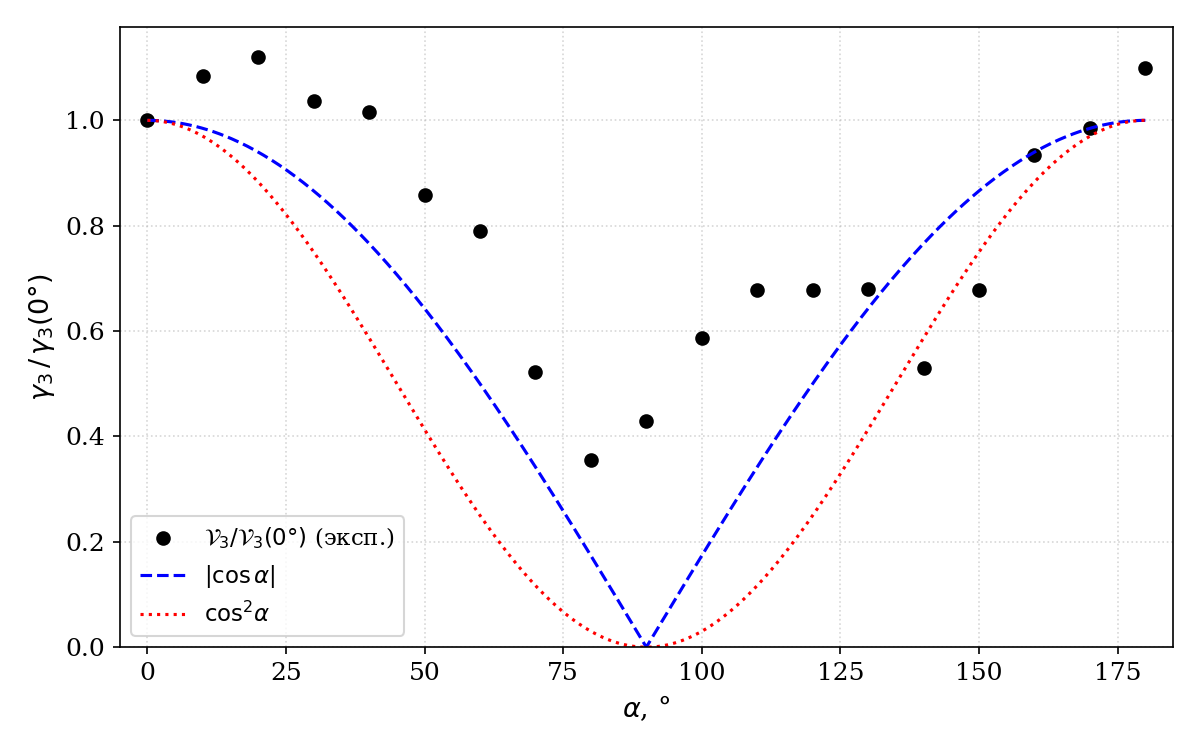
\includegraphics[width=0.82\linewidth]{plot_angle.png}
  \caption{Нормированная $\gamma_3/\gamma_3(0^\circ)$ от угла поляроида. Пунктир~--- $|\cos\alpha|$,
           точки~--- $\cos^2\!\alpha$.}
  \label{fig:angle}
\end{figure}

На рис.~\ref{fig:angle} видно, что экспериментальные точки в целом следуют зависимости $|\cos\alpha|$, что соответствует формуле~\eqref{eq:V3} для линейно поляризованного лазерного излучения. Минимум наблюдается при $\alpha \approx 80^\circ$ (а не при $90^\circ$)~--- смещение объясняется неточностью нулевой риски шкалы поляроида. Значения $\gamma_3/\gamma_3(0^\circ) > 1$ при $\alpha < 50^\circ$ также связаны с этим смещением: истинный максимум $\gamma_3$ соответствует $\alpha \approx 20^\circ$.

\needspace{10\baselineskip}
\subsection*{Измерение \texorpdfstring{$\gamma_2$}{gamma2}: зависимость от разности хода}

Условия: $\alpha = 0$ ($\gamma_3 = 1$). Из~\eqref{eq:vis}: $\gamma_2 = \gamma/\gamma_1$.
Блок~Б$_2$ перемещается от $x = 10$\,см до $x = 88$\,см; разность хода $\ell = 2x$.

\begin{table}[H]
\centering
\caption{Зависимость видности от разности хода ($\alpha = 0$).}
\label{tab:pos}
\footnotesize
\setlength{\tabcolsep}{5pt}
\begin{tabular}{r r r r r r r}
\toprule
$x$,\,см & $\ell$,\,см & $h_1$,\,дел & $h_2$,\,дел & $h_3$,\,дел & $h_4$,\,дел & $\gamma_2$ \\
\midrule
 10 &  20 & 4.0 & 7.5 &  7.0 & 16.0 & 0.411 \\
 12 &  24 & 4.0 & 5.0 &  4.0 & 13.0 & 0.533 \\
 14 &  28 & 4.0 & 3.5 &  3.0 & 11.0 & 0.573 \\
 16 &  32 & 4.0 & 4.5 &  3.0 & 13.0 & \textbf{0.626} \\
 18 &  36 & 4.0 & 3.0 &  3.0 & 10.0 & 0.544 \\
 20 &  40 & 4.0 & 3.5 &  3.5 & 11.0 & 0.518 \\
 22 &  44 & 4.0 & 3.5 &  4.0 & 10.0 & 0.430 \\
 24 &  48 & 4.0 & 1.5 &  3.0 &  6.0 & 0.374 \\
 26 &  52 & 4.0 & 1.5 &  4.0 &  6.0 & 0.225 \\
 28 &  56 & 4.0 & 3.0 &  5.5 &  8.0 & 0.187 \\
 30 &  60 & 4.0 & 2.0 &  4.5 &  6.0 & 0.152 \\
 40 &  80 & 4.0 & 11.0 & 14.0 & 16.0 & \textbf{0.075} \\
 50 & 100 & 4.0 & 4.0 &  6.5 &  8.0 & 0.103 \\
 60 & 120 & 4.0 & 0.5 &  3.5 &  4.0 & 0.106 \\
 70 & 140 & 4.0 & 2.0 &  4.0 &  6.5 & 0.253 \\
 72 & 144 & 4.0 & 4.5 &  6.0 &  9.5 & 0.226 \\
 74 & 148 & 3.5 & 0.5 &  3.0 &  5.0 & 0.378 \\
 76 & 152 & 3.5 & 2.5 &  3.5 &  8.0 & 0.397 \\
 78 & 156 & 3.5 & 2.5 &  3.5 &  8.5 & 0.423 \\
 80 & 160 & 3.5 & 1.5 &  3.0 &  6.0 & 0.364 \\
 82 & 164 & 3.5 & 1.5 &  3.0 &  7.0 & \textbf{0.436} \\
 84 & 168 & 3.5 & 1.5 &  3.0 &  7.0 & 0.436 \\
 86 & 172 & 3.5 & 0.5 &  4.0 &  5.0 & 0.168 \\
 88 & 176 & 3.5 & 1.0 &  3.0 &  4.0 & 0.172 \\
\bottomrule
\end{tabular}
\end{table}

\begin{figure}[H]
  \centering
  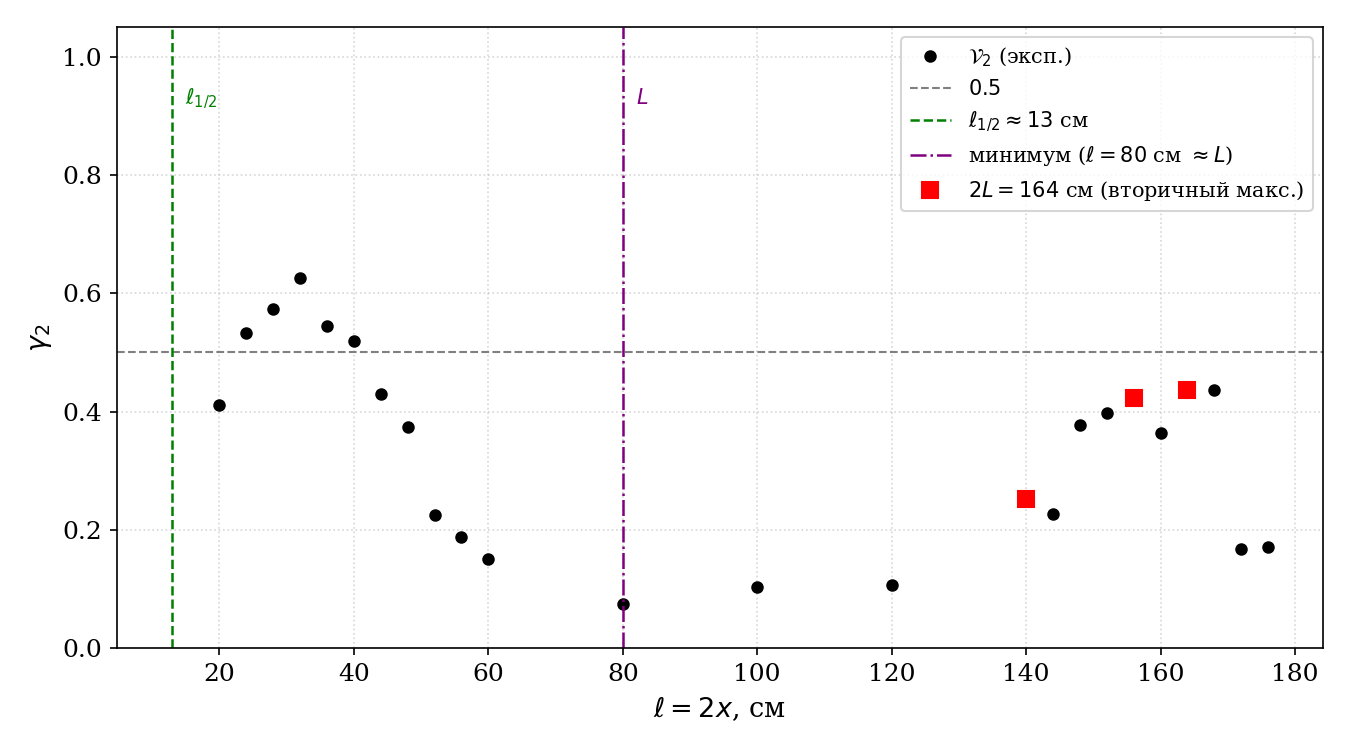
\includegraphics[width=0.90\linewidth]{plot_position.png}
  \caption{Зависимость $\gamma_2$ от разности хода~$\ell = 2x$.
           Красные квадраты~--- вторичный максимум ($\ell = 2L$);
           штрих-пунктир~--- положение минимума ($\ell \approx L$);
           пунктир~--- $\gamma_2 = 0{,}5$.}
  \label{fig:pos}
\end{figure}

\subsection*{Параметры лазера}

\textbf{Длина резонатора.} Глобальный минимум $\gamma_2$ наблюдается при $\ell = 80$\,см ($x = 40$\,см), что отвечает $\ell \approx L$. Вторичный максимум при $\ell = 164$\,см ($x = 82$\,см) соответствует $\ell = 2L$:
\[
  L = \frac{164}{2} = 82 \pm 2\text{\,см}.
\]
Погрешность определяется точностью отсчёта положения блока~Б$_2$ ($\sigma_x = 2$\,см).

\textbf{Межмодовое расстояние:}
\[
  \Delta\nu_m = \frac{c}{2L} = \frac{3 \cdot 10^{10}}{164} = 183 \pm 4\text{\,МГц}.
\]

\textbf{Полуширина $\ell_{1/2}$.}
Поскольку первые точки при $\ell = 20$\,см уже дают $\gamma_2 \approx 0{,}41 < 0{,}5$, значение $\ell_{1/2}$ найдено экстраполяцией сглаживающего сплайна с граничным условием $\gamma_2(0) = 1$:
\[
  \ell_{1/2} \approx 13 \pm 4\text{\,см}
\]
(погрешность оценена консервативно: $\ell_{1/2}$ лежит в интервале $[0;\,20]$\,см).

\textbf{Ширина спектра:}
\[
  \Delta\nu = \frac{0{,}6\,c}{\ell_{1/2}} = \frac{0{,}6 \times 3 \cdot 10^{10}}{13}
  \approx 1{,}4 \pm 0{,}4\text{\,ГГц}.
\]

\textbf{Число мод:}
\[
  n \approx 1 + 1{,}2\,\frac{L}{\ell_{1/2}} = 1 + 1{,}2 \cdot \frac{82}{13}
  \approx 9 \pm 2.
\]

\textbf{Длина когерентности:}
\[
  L_{\text{ког}} = \frac{c}{\Delta\nu} \approx 21 \pm 7\text{\,см}.
\]

Полученные результаты сведены в таблицу~\ref{tab:results}.

\begin{table}[H]
\centering
\caption{Итоговые параметры лазера.}
\label{tab:results}
\begin{tabular}{l l}
\toprule
Величина & Значение \\
\midrule
Длина резонатора $L$ & $(82 \pm 2)$\,см \\
Межмодовое расстояние $\Delta\nu_m$ & $(183 \pm 4)$\,МГц \\
Полуширина гл. максимума $\ell_{1/2}$ & $(13 \pm 4)$\,см \\
Ширина спектра $\Delta\nu$ & $(1{,}4 \pm 0{,}4)$\,ГГц \\
Число продольных мод $n$ & $9 \pm 2$ \\
Длина когерентности $L_{\text{ког}}$ & $(21 \pm 7)$\,см \\
\bottomrule
\end{tabular}
\end{table}

\section*{Вывод}

В работе исследована видность интерференционной картины He-Ne-лазера в интерферометре Майкельсона:

\begin{enumerate}
  \item Зависимость $\gamma_3$ от угла поляроида~$\alpha$ подтверждает формулу
        $\gamma_3 = |\cos\alpha|$: лазер генерирует линейно поляризованное излучение.
  \item Зависимость $\gamma_2(\ell)$ показала минимум при $\ell \approx L = 82$\,см и
        вторичный максимум при $\ell = 2L = 164$\,см. Межмодовое расстояние
        $\Delta\nu_m \approx 183$\,МГц. Ширина спектра $\Delta\nu \approx 1{,}4$\,ГГц
        согласуется с допплеровским уширением линии неона (${\approx}1{,}5$\,ГГц).
        Лазер генерирует $n \approx 9$ продольных мод; длина когерентности
        $L_{\text{ког}} \approx 21$\,см.
\end{enumerate}

\begin{thebibliography}{99}
\bibitem{labmanual}
Лабораторный практикум по общей физике. Т.\,2. Оптика / А.\,В.~Максимычев и~др.;
под ред. А.\,В.~Максимычева.~--- М.: МФТИ, 2014.~--- 446\,с.
\end{thebibliography}

\end{document}
